%=============================================================================
% A Bit-Accurate Power-of-Two INT8 1D-CNN Accelerator for ECG Arrhythmia
% Classification on a Cyclone V FPGA
%
% Condensed from: 22200034_Thesis_EN.docx (Le Minh Duc, HCMUS, 2026)
% Class: IEEEtran conference, two-column, target 6 pages.
% Build:  pdflatex ecg_fpga_paper.tex  (x2 for cross-references)
%=============================================================================
\documentclass[conference,10pt]{IEEEtran}

\usepackage{cite}
\usepackage{amsmath,amssymb}
\usepackage{graphicx}
\graphicspath{{figures_paper/}}
\usepackage{subcaption}
\usepackage{booktabs}
\usepackage{array}
\usepackage[T1]{fontenc}
\usepackage[utf8]{inputenc}
\usepackage{url}

% Compact tables/figures so the paper holds 6 pages
\renewcommand{\arraystretch}{1.05}
\setlength{\textfloatsep}{8pt plus 2pt minus 2pt}
\setlength{\floatsep}{8pt plus 2pt minus 2pt}
\setlength{\intextsep}{8pt plus 2pt minus 2pt}

\begin{document}

\title{A Bit-Accurate Power-of-Two INT8 1D-CNN Accelerator\\
for ECG Arrhythmia Classification on a Cyclone~V FPGA}

\author{\IEEEauthorblockN{Le Minh Duc}
\IEEEauthorblockA{Faculty of Electronics and Telecommunications\\
University of Science, VNU-HCM\\
Ho Chi Minh City, Vietnam\\
22200034@student.hcmus.edu.vn}
\and
\IEEEauthorblockN{Ma Khai Minh}
\IEEEauthorblockA{Faculty of Electronics and Telecommunications\\
University of Science, VNU-HCM\\
Ho Chi Minh City, Vietnam}}

\maketitle

\begin{abstract}
Continuous arrhythmia monitoring on wearable devices requires a classifier that
is accurate, deterministic in latency and frugal in area and energy. This paper
presents an FPGA accelerator for four-class rhythm classification from
single-lead ECG. A four-layer 1D-CNN is channel-pruned to 640 parameters and
quantized to INT8 with power-of-two scaling, so that requantization reduces to a
constant addition and a bit shift and consumes no hard multiplier. Two design
decisions distinguish the work from earlier shift-based ECG accelerators. First,
rescaling uses round-half-up instead of the customary arithmetic right shift,
making the quantization error symmetric about zero at identical hardware cost.
Second, correctness is established by bit-accurate comparison against a reference
integer model at seven checkpoints spanning the whole network, rather than by
aggregate accuracy, which can hide mutually cancelling deviations. The core
time-multiplexes one engine of eight parallel convolution--pool units across the
four layers. On a Cyclone~V 5CSXFC6D6F31C6 it occupies 2{,}148 ALMs (5\%), 28 DSP
blocks (25\%) and 20 M10K blocks (4\%), closes timing at 108.86~MHz, and completes
one inference in a fixed 5{,}216 cycles (52.16~$\mu$s at 100~MHz, 19{,}172
inferences/s). It reaches 94.27\% accuracy and 0.9356 macro-F1 on the Chapman
test set, and 93.00\% zero-shot on the Georgia cross-dataset test set. The
bitstream running on a DE10-Standard kit reproduces both figures exactly.
\end{abstract}

\begin{IEEEkeywords}
ECG classification, 1D-CNN, INT8 quantization, power-of-two scaling, bit-accurate
verification, FPGA, Cyclone~V, hardware accelerator.
\end{IEEEkeywords}

%=============================================================================
\section{Introduction}
%=============================================================================

Cardiac arrhythmia is a leading cause of sudden cardiac death. Many arrhythmias,
atrial fibrillation being the most representative, are paroxysmal: they occur
intermittently and may go undetected during a single examination at a medical
facility. What is needed is automated monitoring running directly on a wearable
or edge device.

Convolutional neural networks classify arrhythmias from ECG with accuracy
approaching that of cardiologists \cite{hannun2019}, but high-performance models
carry many parameters: microcontrollers lack the real-time throughput, while GPUs
exceed the power and size budget of a wearable. The obstacle is therefore not a
still more accurate model, but fitting an already accurate model into an
acceptable device form. When layer count, kernel sizes and channel counts are
fixed in advance, a circuit can follow the network structure closely, keep every
weight on chip and omit the control logic needed only for generality. An FPGA
suits such a circuit: it offers parallelism at the arithmetic level, gives
deterministic latency, and lets area, frequency and power be measured on real
hardware.

Two aspects of the usual design practice deserve revisiting. Power-of-two scaling
is attractive because requantization degenerates into a bit shift, but it is
normally realized with an arithmetic right shift, which always rounds towards
negative infinity; the resulting error is one-sided and accumulates across
layers. Separately, quantized accelerators are commonly validated by comparing
aggregate test accuracy against the software model, a check that two errors of
opposite sign can pass.

This paper makes three contributions:

\begin{itemize}
\item \textbf{Quantization.} Power-of-two INT8 quantization-aware training in
which rescaling rounds half-up rather than truncating, keeping the error
symmetric about zero at the cost of one constant addition and no DSP block
(Section~\ref{sec:quant}).
\item \textbf{Verification.} A bit-accurate methodology comparing the circuit
against a reference integer model at seven checkpoints throughout the network,
requiring exact agreement at every stage rather than at the output alone
(Section~\ref{sec:verif}).
\item \textbf{Deployment.} A complete area-frugal core, synthesized, timed,
power-analyzed and run on a DE10-Standard kit over two full test sets, including
a zero-shot cross-dataset evaluation on data from a different acquisition system
(Sections~\ref{sec:arch} and \ref{sec:results}).
\end{itemize}

%=============================================================================
\section{Related Work}
%=============================================================================

Kiranyaz \emph{et al.} \cite{kiranyaz2016} showed that a shallow 1D-CNN
classifies heartbeats in real time with competitive accuracy; later work extended
this to deep networks at cardiologist level \cite{hannun2019} or took the
opposite path of compacting the model for wearables \cite{le2023}. Working
directly on the sample sequence costs far less computation than converting the
ECG into an image and applying a 2D CNN \cite{yoon2023}.

On the hardware side, Sze \emph{et al.} \cite{sze2017} classify accelerators
along two axes: how parallelism is exploited, and how layers map onto hardware. A
fully mapped design dedicates hardware to every layer and pipelines them, giving
high throughput at an area cost that grows with depth, with the slowest layer
setting the system rate \cite{venieris2018}. Liu \emph{et al.} \cite{liu2023}
follow this route for ECG on a Cyclone~V, reaching 66~$\mu$s per inference while
occupying 51\% of the ALMs and 86\% of the registers, and rescale by arithmetic
shift. Pham \emph{et al.} \cite{pham2025} implement a flexible processing-element
array on a large Zynq UltraScale+ device, and Tran \emph{et al.} \cite{tran2026}
use low-dimensional hypervector computing without DSP blocks; both classify
individual beats on MIT-BIH.

For a model whose weights fit entirely on chip, bandwidth is not the bottleneck
\cite{zhang2015}, so logic and energy are what must be minimized. A further trait
of 1D networks with pooling is that the data shape varies markedly across
layers---the first layer processes a long sequence with few channels, the last a
short one with many---so the dimension chosen for parallelism must be the one
that varies least, or the hardware idles. These two observations lead to the
single-engine, time-shared organization adopted here, parallel over output
channels and over the weights within a kernel.

%=============================================================================
\section{Model and Quantization}
\label{sec:quant}
%=============================================================================

The software stage produces a compact, accurate INT8 weight set in the exact
layout the hardware expects, through the sequence of Fig.~\ref{fig:swflow}.

\begin{figure}[t]
\centering
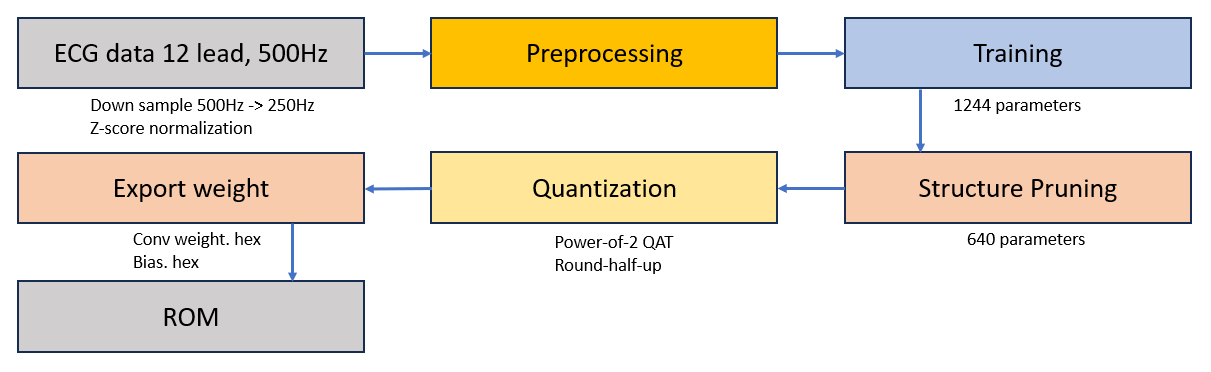
\includegraphics[width=\columnwidth]{fig_swflow.png}
\caption{Software flow from the raw 12-lead recordings to the weight files loaded
into the on-chip ROMs.}
\label{fig:swflow}
\end{figure}

\subsection{Datasets and Preprocessing}

Training and in-distribution evaluation use Chapman \cite{zheng2020}, a
consolidation of two related PhysioNet collections of 12-lead, 10~s, 500~Hz
records with physician-assigned rhythm labels. After removing records duplicated
between the two sources to avoid leakage, 33{,}143 records remain. The detailed
diagnostic codes are grouped into four classes following the taxonomy of the
dataset authors: AFIB (atrial fibrillation, atrial flutter), GSVT
(supraventricular tachycardias), SB (sinus bradycardia) and SR (sinus rhythm,
sinus irregularity). Only lead~II is used, the lead whose axis nearly matches
impulse propagation from the sinus node to the apex. Each record is resampled
from 500 to 250~Hz, giving 2{,}500 samples per 10~s window, and Z-score
normalized. The split is 70/15/15 and patient-independent: records of one patient
never appear in two subsets, giving 23{,}198 training, 4{,}972 validation and
4{,}973 test records. Fig.~\ref{fig:ecg} shows one record of each class, with the
differences in rate and R--R regularity the network must learn.

\begin{figure}[t]
\centering
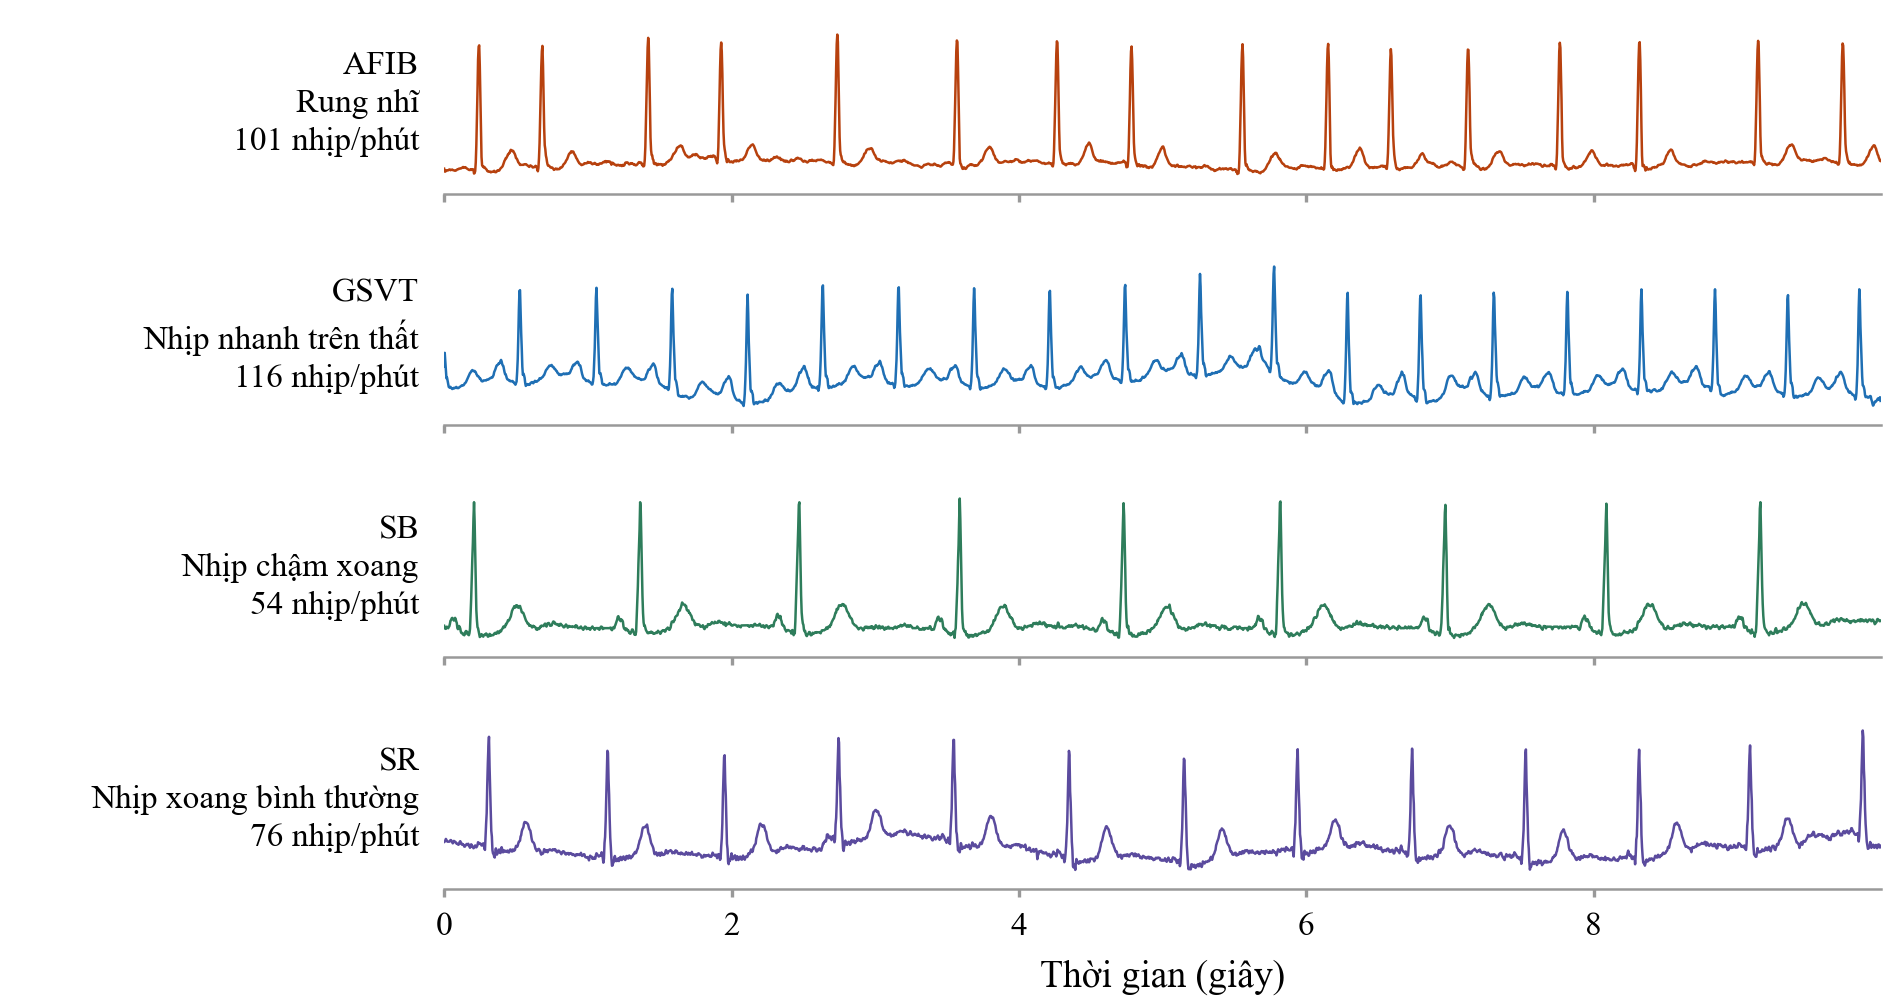
\includegraphics[width=\columnwidth]{fig_ecg.png}
\caption{Typical lead-II waveforms of the four rhythm classes; each trace is one
10-second record from the test set.}
\label{fig:ecg}
\end{figure}

The cross-dataset test set is the Georgia 12-lead ECG Challenge Database
\cite{alday2020}, collected at a different institution with an entirely different
recording system and sharing no records with the training data, so it constitutes
a far-transfer test. Records mapping unambiguously onto the four classes were
kept, yielding 5{,}459 records used for evaluation only.

The task is posed as whole-record classification: each fixed-length window
receives one of the four labels, rather than classifying beats after R-peak
detection. This removes the noise-sensitive segmentation stage, which would need
separate hardware, and lets the circuit work on a continuous sample stream.

\subsection{Network and Pruning}

The network is a 1D-CNN of four convolutional layers, each with kernel $K=5$ and
padding $P=2$ followed by max-pooling of window and stride 5, ending in global
average pooling (GAP) and a fully connected (FC) layer over four classes. ReLU is
applied after Conv4 only: for images the negative part carries little
information, but in the ECG it is physiologically real, the Q and S waves being
negative deflections of the QRS complex, so Conv1--Conv3 preserve sign.

The trained model has the channel configuration $(4,8,8,16)$ and 1{,}244
parameters. Structured channel pruning by $L_1$ filter norm \cite{li2017} removes
whole filters, which genuinely shrinks the tensors and hence the multipliers and
memory needed---unlike unstructured pruning, whose sparse matrix yields a benefit
only if the hardware can skip zeros. Fine-tuning follows in two phases, 30 epochs
at learning rate $10^{-3}$ and 20 at $10^{-4}$. The result is the configuration
$(4,4,8,8)$ with 640 parameters, 48.55\% fewer, and is the configuration
implemented in hardware (Fig.~\ref{fig:model}). Table~\ref{tab:layers} gives the
layer shapes.

\begin{figure*}[t]
\centering
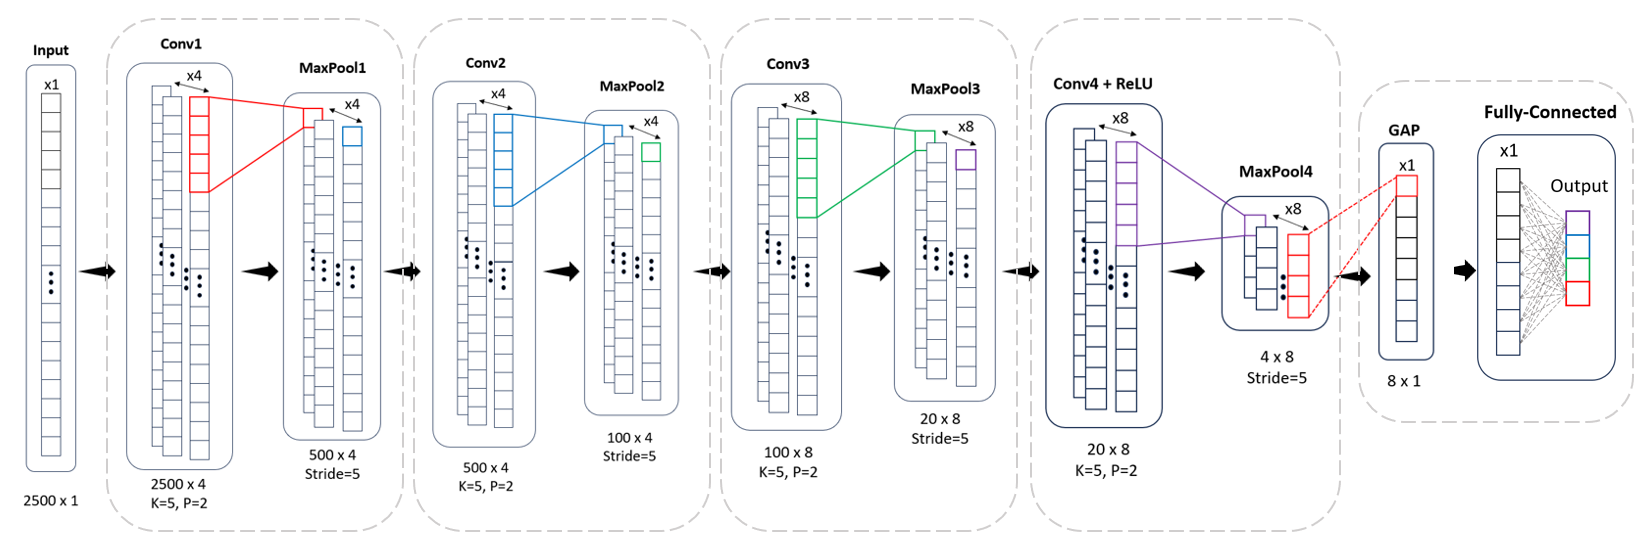
\includegraphics[width=\textwidth]{fig_model.png}
\caption{The pruned 1D-CNN implemented in hardware (640 parameters). Each
convolutional layer uses $K=5$, $P=2$ and is followed by max-pooling of window
and stride 5; ReLU is applied after Conv4 only.}
\label{fig:model}
\end{figure*}

\begin{table}[t]
\caption{Layer configuration of the pruned model (640 parameters).}
\label{tab:layers}
\centering
\footnotesize
\begin{tabular}{lccccrr}
\toprule
Layer & $C_{\text{in}}$ & $C_{\text{out}}$ & Pool & ReLU & Output & Par. \\
\midrule
Conv1 & 1 & 4 & /5 & No  & $4\times500$ & 24 \\
Conv2 & 4 & 4 & /5 & No  & $4\times100$ & 84 \\
Conv3 & 4 & 8 & /5 & No  & $8\times20$  & 168 \\
Conv4 & 8 & 8 & /5 & Yes & $8\times4$   & 328 \\
GAP   & 8 & 8 & /4 & --- & $8\times1$   & 0 \\
FC    & 8 & 4 & --- & --- & $4$         & 36 \\
\midrule
Total & & & & & & \textbf{640} \\
\bottomrule
\end{tabular}
\end{table}

\subsection{Power-of-Two Quantization with Round-Half-Up}

Quantization represents a floating-point tensor as INT8 values times a scale
factor \cite{jacob2018}. Constraining that factor to a power of two
\cite{miyashita2016} turns the division by it into a right shift---on an FPGA
merely a rewiring of bits---whereas a general factor needs one DSP block per
rescaling. For a tensor $T$ the shift coefficient is

\begin{equation}
\text{shift\_bits}(T) = \left\lfloor \log_2 \frac{127}{\max|T|} \right\rfloor ,
\end{equation}

the largest power of two that preserves the full range of $T$ without clipping at
the boundary. The inference pipeline, identical in the Python reference and in
the circuit, is

\begin{align}
x_q &= \mathrm{clamp}\!\left(\mathrm{round}(x \cdot 2^{s_{\text{in}}}),\,-127,\,127\right), \\
w_q &= \mathrm{clamp}\!\left(\mathrm{round}(w \cdot 2^{s_w}),\,-127,\,127\right), \\
\mathrm{acc} &= \textstyle\sum x_q w_q + b_{\text{scaled}},\qquad
b_{\text{scaled}} = \mathrm{round}(b\cdot 2^{nb}),
\end{align}

with the accumulation in INT32 and the bias carried at the accumulator scale, not
the weight scale, for the addition to be dimensionally valid. Rescaling to the
INT8 input range of the next layer is

\begin{equation}
\label{eq:rhu}
\mathrm{out} = \mathrm{clamp}\!\left( \frac{\mathrm{acc} + 2^{\,nb-1}}{2^{\,nb}},\,
-127,\,127 \right),
\end{equation}

where the division is an arithmetic right shift by $nb$ bits. The additive
constant $2^{nb-1}$ is the whole point of \eqref{eq:rhu}: a bare arithmetic shift
always rounds towards $-\infty$, so its error is one-sided and biases every
subsequent layer in the same direction, whereas adding half the unit of the
shifted-out bit rounds to the nearest integer and leaves the error symmetric
about zero. The cost is one constant addition, and in the implementation even
that disappears, being merged into the accumulator initialization
(Section~\ref{sec:cp}). Quantization-aware training is used, with the
straight-through estimator \cite{bengio2013} for the zero derivative of rounding.
Table~\ref{tab:qparams} lists the calibrated coefficients; $nb=0$ at the FC
layer, whose raw INT32 logits feed argmax directly, softmax being monotone and
hence unnecessary at inference.

\begin{table}[t]
\caption{Power-of-two quantization coefficients per layer.}
\label{tab:qparams}
\centering
\footnotesize
\begin{tabular}{lccl}
\toprule
Layer & $s_w$ & $nb$ & Remark \\
\midrule
Conv1 & 6 & 8 & $nb = s_{\text{in}} + s_w = 2+6$ \\
Conv2 & 7 & 7 & input already INT8, $nb=s_w$ \\
Conv3 & 6 & 6 & input already INT8, $nb=s_w$ \\
Conv4 & 7 & 7 & input already INT8, $nb=s_w$ \\
FC    & 7 & 0 & no rescaling; raw logits to argmax \\
\bottomrule
\end{tabular}
\end{table}

Weights are exported with the output channel outermost and the input channel
innermost, the five weights of an (output channel, input channel) pair packed
into one 40-bit word. This matches the hardware exactly: each unit handles one
output channel and needs, each cycle, the five weights of one input channel, in a
single access with no run-time byte assembly.

%=============================================================================
\section{Hardware Architecture}
\label{sec:arch}
%=============================================================================

The core uses one shared computational engine, time-multiplexed across the four
layers under a single finite state machine, rather than unrolling the layers into
four hardware blocks. With only 640 parameters a fully unrolled design would
leave the Conv1 hardware---one input channel---idle most of the time, whereas
reusing the engine keeps the area low while still meeting the latency required
for continuous monitoring. The design comprises the engine unit (eight parallel
convolution--pool units and the data-supply mechanism), the gap-fc-argmax unit,
the controller, a two-bank ping-pong feature-map memory and the input memory, as
shown in Fig.~\ref{fig:arch}.

\begin{figure}[t]
\centering
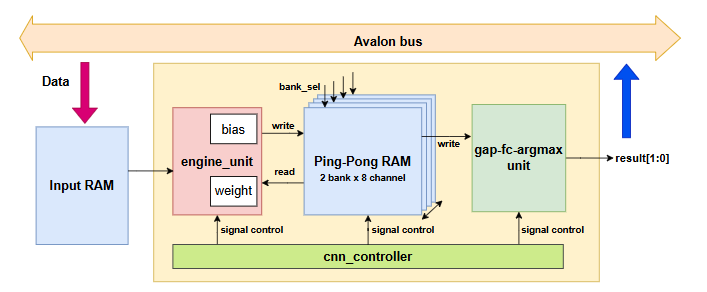
\includegraphics[width=\columnwidth]{fig_arch.png}
\caption{Top-level organization of the accelerator. One engine is time-shared
across the four convolutional layers, reading one ping-pong bank and writing the
other.}
\label{fig:arch}
\end{figure}

\subsection{Convolution--Pool Unit}
\label{sec:cp}

\begin{figure}[t]
\centering
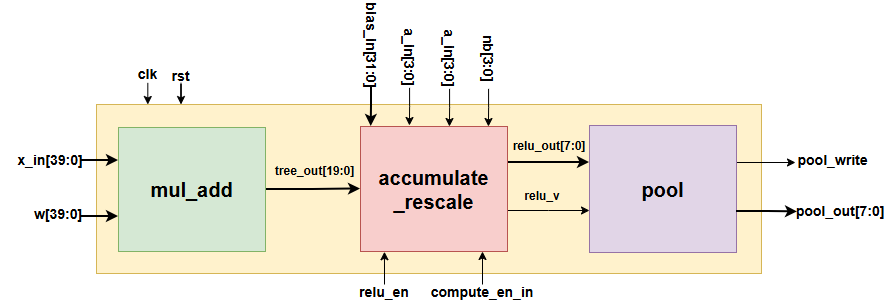
\includegraphics[width=\columnwidth]{fig_cpunit.png}
\caption{The convolution--pool unit and its three sub-blocks. The split is
structural and does not alter the arithmetic.}
\label{fig:cpunit}
\end{figure}

The convolution--pool unit (Fig.~\ref{fig:cpunit}) is the elementary compute
element and handles one output channel. Each cycle it takes a window of five
samples with the five matching weights, performs the convolution, rescales to
INT8 and applies max-pooling. It is a nine-stage pipeline: five signed $8\times8$ multiplications
(S1); a three-stage registered adder tree (S2--S4); multi-channel accumulation
(S5); a latching stage (S\textsubscript{bias}); the rescaling shift (S6);
saturation to $[-127,127]$ (S7); ReLU, effective in Conv4 only (S8); and
max-pooling over a window of five (S9).

At S5 the bias and the rounding constant of \eqref{eq:rhu} are merged into the
initialization term of the accumulator instead of being added at later stages.
By associativity of addition the transformation is exactly bit-accurate with
$(\mathrm{acc}+b+2^{nb-1}) \gg nb$, and all intermediate bounds lie safely inside
the signed 32-bit range, so the round-half-up correction costs no adder of its own
on the critical path. Stage S9 holds a comparator and a counter from 0 to 4: the
first valid value enters the maximum register, later values update it only if
larger, and on the fifth the block asserts \texttt{pool\_write}. The counter is
gated by compute-enable so that it ignores the spurious values produced while the
window is priming.

\subsection{Engine Unit}

\begin{figure*}[t]
\centering
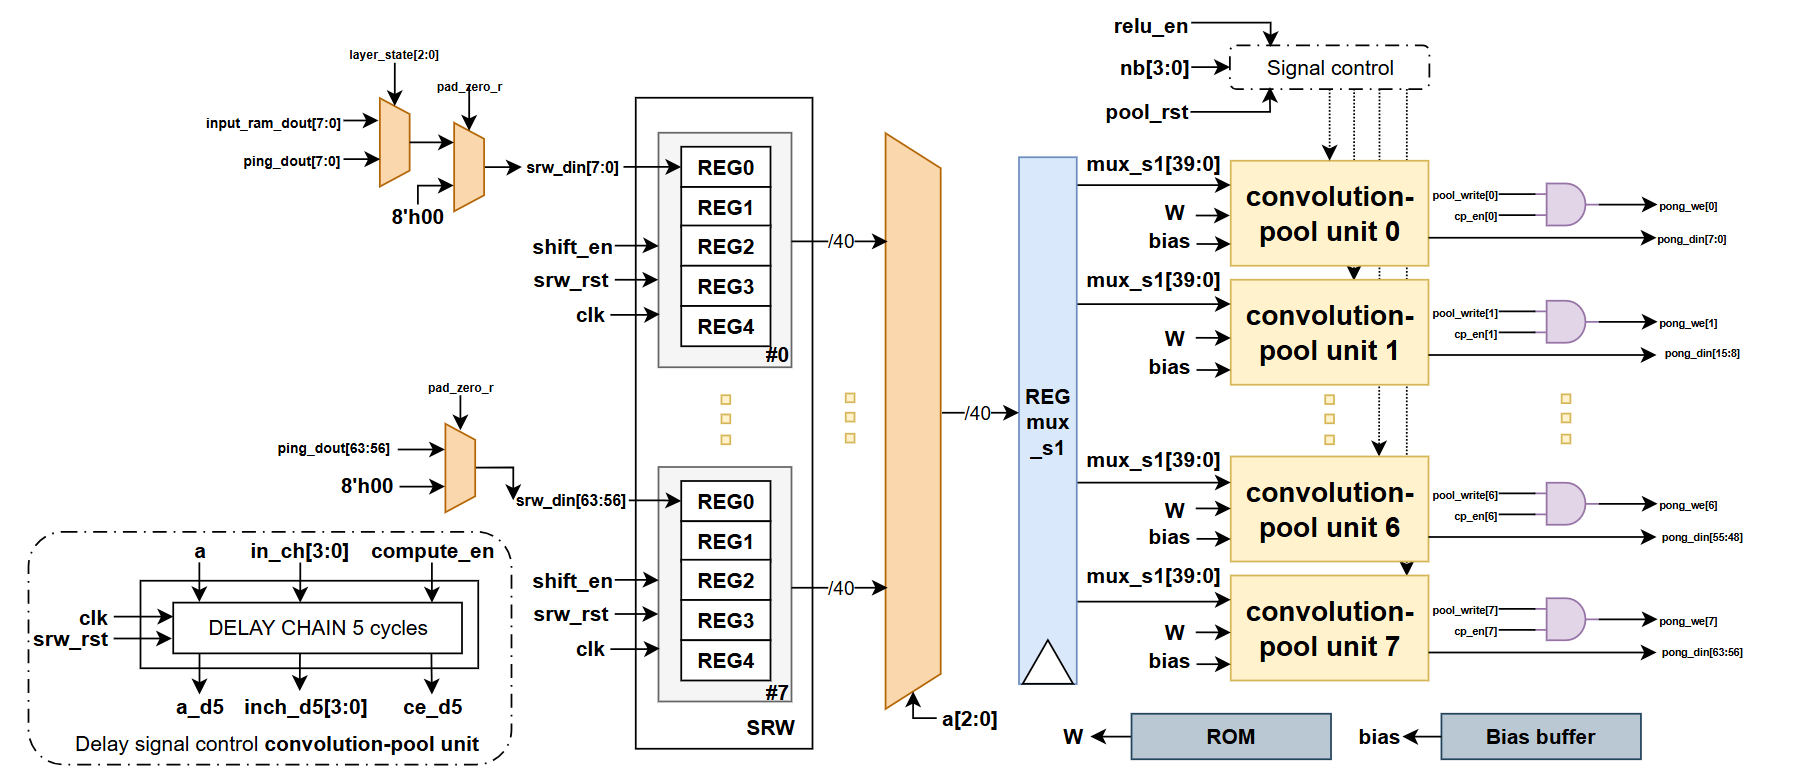
\includegraphics[width=\textwidth]{fig_engine.png}
\caption{Engine unit. Eight sliding register windows (SRW) feed a shared branch
selector, whose output drives the eight convolution--pool units in parallel; the
five-cycle delay chain (lower left) realigns the channel counter, the layer
channel count and compute-enable with the accumulator update at the end of the
pipeline.}
\label{fig:engine}
\end{figure*}

The engine unit (Fig.~\ref{fig:engine}) places eight convolution--pool units in
parallel, computing eight output channels at once, and holds the mechanism that
feeds them: a sliding register window, the branch selector, the delay chains, the
weight store and the per-channel write ports. Parallelism is thus over output
channels and over the five taps within a kernel, the two dimensions that vary
least across layers.

Each input channel has a five-cell shift register. Computed directly, each sample
would be read five times, belonging as it does to five consecutive output
windows; with the sliding window each sample is read exactly once and then slides
through all five positions, cutting memory traffic to one fifth. Eight such
windows are provided, enough for Conv4, the layer with the most input channels.
Convolution with $P=2$ needs the two positions at each end treated as zero, so a
padding flag is asserted when the read address falls below 2 or reaches
$L_{\text{in}}+2$; the flag passes through a register stage before use, because
on-chip memory has one cycle of synchronous read latency and an unregistered flag
would place the zeros one position early.

The pipeline from branch selector to accumulator register is exactly five cycles
deep: selection and weight-address issue at cycle $N$, the registered window and
weight word at $N{+}1$, the multiplications at $N{+}2$, the adder tree at
$N{+}3$ and $N{+}4$, and the accumulator update at $N{+}5$. The control signals
that qualify that update---the input-channel counter, the layer channel count and
compute-enable---therefore cannot be taken from the head of the pipeline, where
they have already moved on. Each is delayed through a five-stage shift chain, and
only the final stage is wired to the eight units. The depth must match the real
pipeline exactly: an error of one cycle attributes every convolution sum to the
wrong input channel, shifts the max-pooling window, and makes every result from
that layer onwards diverge from the reference.

\subsection{GAP--FC--Argmax Unit and Controller}

The gap-fc-argmax unit performs the last three steps as a sub-state machine of 22
cycles: 6 for GAP, 10 for FC, 1 flush cycle, 4 for argmax and 1 to latch the
result. GAP sums the four remaining Conv4 outputs of each channel and divides by
four; since the input has passed ReLU, this is a right shift by two bits, an
integer floor division that the reference model reproduces exactly. The FC stage
uses four parallel multipliers, one per output class, scanning the eight inputs
through a two-stage pipeline with the bias preloaded into the accumulator, so it
is added at no extra cost; the two cycles of pipeline latency are why one flush
cycle is needed. Argmax compares the four logits over four cycles with one
register for the maximum and one for its index.

\begin{table}[t]
\caption{States of the controller.}
\label{tab:fsm}
\centering
\footnotesize
\begin{tabular}{llp{4.5cm}}
\toprule
State & Code & Role \\
\midrule
IDLE       & 0 & Await a command; \texttt{busy} deasserted \\
LOAD\_INPUT & 1 & Load Conv1 parameters, clear window and pooling counters \\
CONV1      & 2 & Layer 1, reading from the input memory \\
CONV2      & 3 & Layer 2 \\
CONV3      & 4 & Layer 3 \\
CONV4      & 5 & Layer 4, ReLU enabled \\
GAP\_FC     & 6 & Global average pooling, FC and argmax \\
DONE       & 7 & Latch the result, issue the \texttt{done} pulse \\
\bottomrule
\end{tabular}
\end{table}

The controller is a single unified state machine over the eight states of
Table~\ref{tab:fsm}, encoded in 3 bits, driving both the engine and the output
classifier, so that all timing sits in one place. Within a convolutional
state two nested counters run: the input-channel counter $a$ from 0 to
$C_{\text{in}}-1$, and the output-position counter $t$, incremented each time $a$
wraps, at which point the window shifts. The engine therefore spends exactly
$C_{\text{in}}$ cycles on each output position, one input channel per cycle,
matching the multi-channel accumulation. Per-layer parameters---input channels,
lengths, $nb$, ReLU enable and the output-channel mask---are reloaded at each
transition; in this single-load design they are constants indexed by layer. The
feature maps live in a two-bank ping-pong memory, each layer reading one bank and
writing the other with the bank select toggling at every transition. Weights sit
in on-chip ROM, so the configuration is fixed at synthesis. The core is wrapped
by an Avalon-MM slave; on the board a JTAG-to-Avalon bridge lets a host script
write the ECG samples, assert start, and read back \texttt{done} and the class
index.

%=============================================================================
\section{Verification Methodology}
\label{sec:verif}
%=============================================================================

Verification proceeds at three levels, each with its own testbench.

At block level, a single convolution--pool unit is driven directly, bypassing the
delay chains of the engine, over 23 cases covering the basic datapath, rounding,
saturation at exactly $\pm127$, ReLU on and off, max-pooling at every window
position and over consecutive windows, accumulation over 4 and 8 channels, idle
cycles and reset. All 23 pass. One case is diagnostic of the rounding
contribution: with bias 128 and $nb=8$, round-half-up gives 1 where truncation
gives 0.

At layer level, engine, controller and ping-pong memory are integrated to check
control and timing across the Conv1$\rightarrow$Conv2$\rightarrow$Conv3
transitions: absence of write pulses during the priming cycles, the write address
at the last pulse of Conv1, the pulse count per layer, the state transitions, the
bank swap and the channel masks. All 8 cases pass. The priming-inhibition case is
what exposes the one-cycle misalignment discussed above.

At system level, a real ECG record is written into the input memory over the bus
and one full inference is run, with the values compared against the reference
integer model at seven checkpoints: the 2{,}500 input samples, the outputs of the
four pooling stages (2{,}000, 400, 160 and 32 values), the 8 GAP values and the 4
FC logits. All seven agree bit for bit, with a maximum absolute deviation of zero
(Fig.~\ref{fig:wave}).

\begin{figure}[t]
\centering
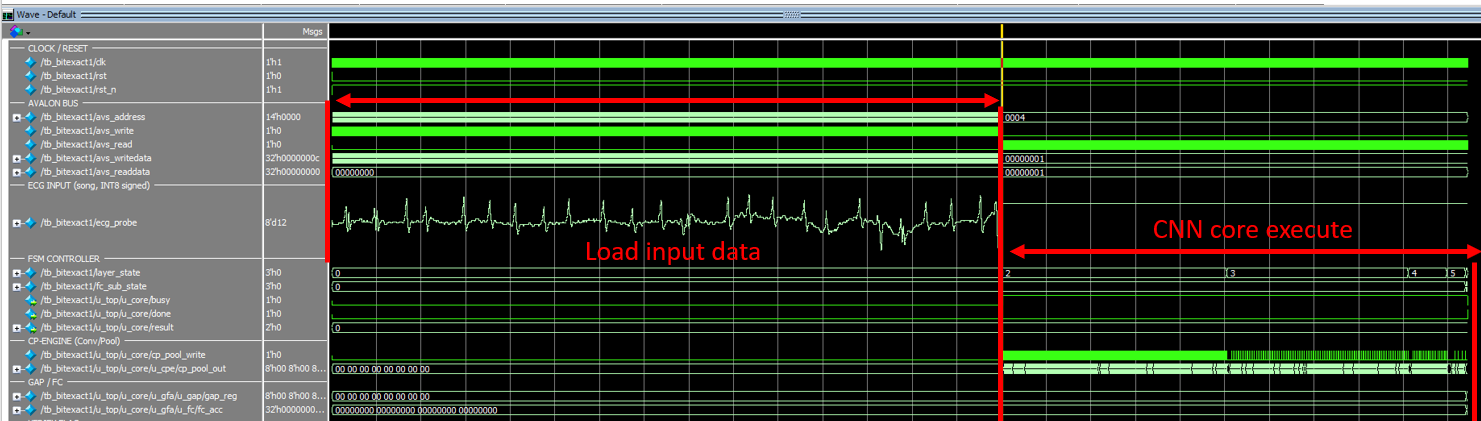
\includegraphics[width=\columnwidth]{fig_sim_bitexact.png}
\caption{Simulation of one complete inference, with the seven checkpoints
compared against the reference integer model.}
\label{fig:wave}
\end{figure}
Because agreement is exact at every stage and not only at the output, the
circuit demonstrably implements the quantization specification itself, with no
mutually cancelling errors---a claim that aggregate accuracy cannot support. The
same environment run with a Georgia record, the ROMs still holding the Chapman
coefficients, likewise matches the reference.

%=============================================================================
\section{Results}
\label{sec:results}
%=============================================================================

\subsection{Classification Accuracy}

\begin{figure}[t]
\centering
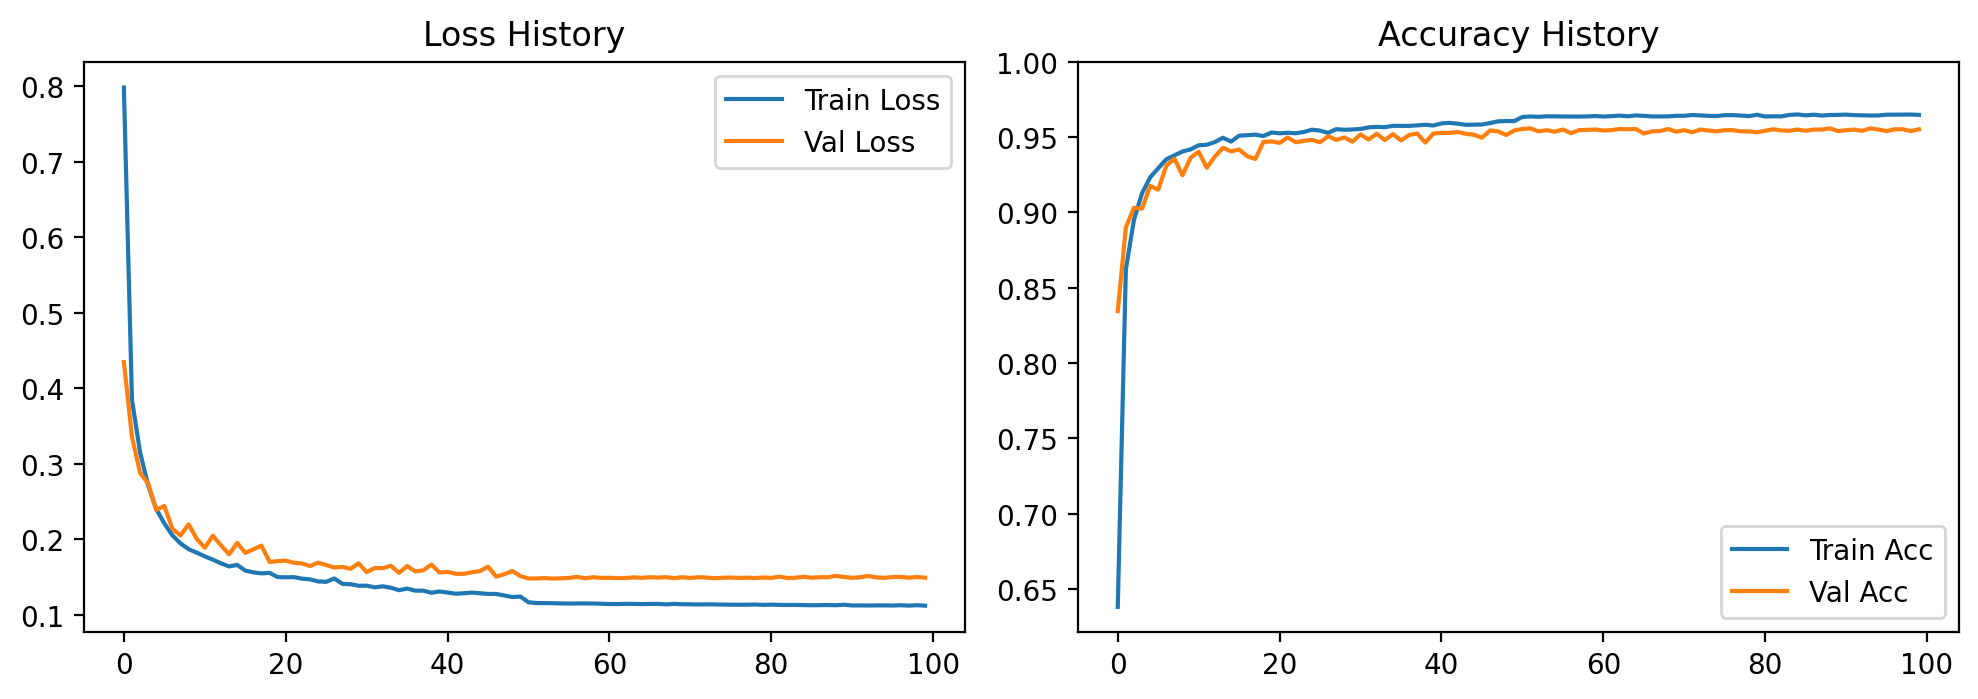
\includegraphics[width=\columnwidth]{fig_train.png}
\caption{Loss and accuracy over training. Validation accuracy tracks training
accuracy about one point behind and stays stable, so the model is not
overfitting.}
\label{fig:train}
\end{figure}

Training converges within the first 20 epochs and then flattens
(Fig.~\ref{fig:train}). Table~\ref{tab:acc} traces accuracy through the
compression steps on the Chapman test set of 4{,}973 records. Pruning removes 48.55\% of the parameters for 0.32
percentage points of accuracy. Quantization costs a further 0.76 points and 0.90
points of macro-F1; agreement between the INT8 and float32 predictions is 0.9761.
The INT8 row is evaluated bit-accurately and is therefore exactly what the
hardware produces.

\begin{table}[t]
\caption{Accuracy through the compression steps (Chapman test set).}
\label{tab:acc}
\centering
\footnotesize
\begin{tabular}{lcccc}
\toprule
Model version & Param. & Acc. (\%) & macro-F1 & macro-AUC \\
\midrule
Float32, unpruned      & 1{,}244 & 95.35 & 0.9478 & --- \\
Float32, pruned        & 640 & 95.03 & 0.9446 & 0.9938 \\
\textbf{INT8, bit-accurate} & \textbf{640} & \textbf{94.27} & \textbf{0.9356} & 0.9712 \\
\bottomrule
\end{tabular}
\end{table}

\begin{table}[t]
\caption{Per-class results of the INT8 model.}
\label{tab:perclass}
\centering
\footnotesize
\begin{tabular}{lccc@{\hskip 10pt}ccc}
\toprule
& \multicolumn{3}{c}{Chapman (in-distribution)} & \multicolumn{3}{c}{Georgia (zero-shot)} \\
\cmidrule(r){2-4}\cmidrule(l){5-7}
Class & Prec. & Rec. & F1 & Prec. & Rec. & F1 \\
\midrule
AFIB & 0.9267 & 0.9062 & 0.9163 & 0.8309 & 0.8237 & 0.8273 \\
GSVT & 0.8698 & 0.9459 & 0.9063 & 0.9208 & 0.9455 & 0.9329 \\
SB   & 0.9756 & 0.9810 & 0.9783 & 0.9537 & 0.9625 & 0.9581 \\
SR   & 0.9670 & 0.9172 & 0.9414 & 0.9513 & 0.9328 & 0.9420 \\
\midrule
Macro & --- & --- & \textbf{0.9356} & --- & --- & \textbf{0.9151} \\
\bottomrule
\end{tabular}
\end{table}

\begin{figure}[t]
\centering
\begin{subfigure}{0.49\columnwidth}
  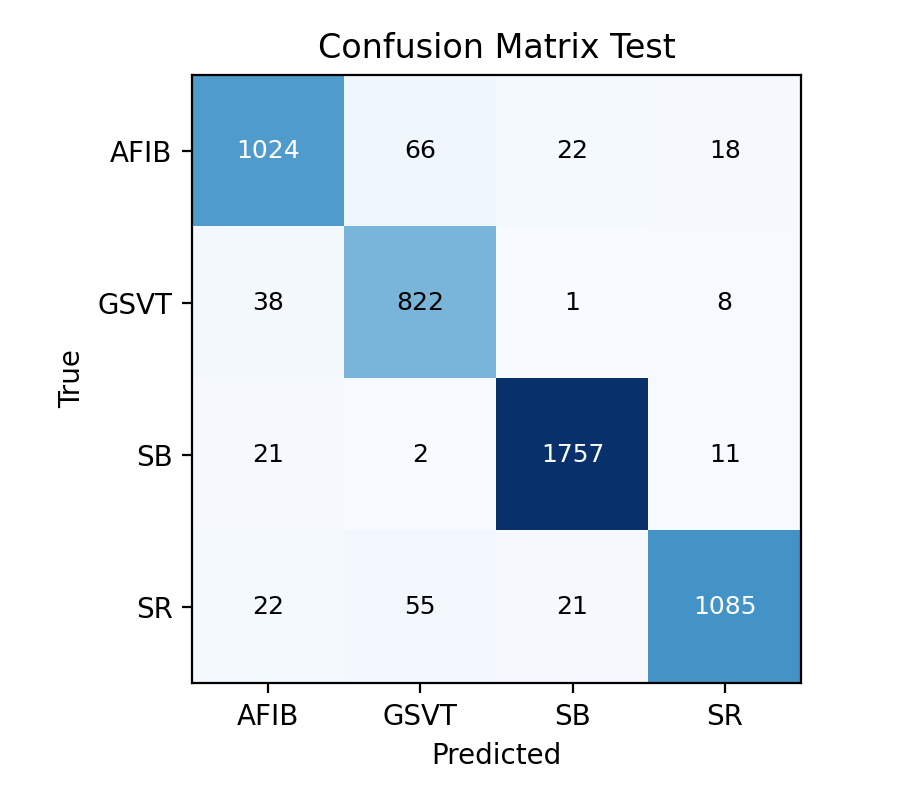
\includegraphics[width=\linewidth]{fig_cm_chapman.png}
  \caption{}
\end{subfigure}
\hfill
\begin{subfigure}{0.49\columnwidth}
  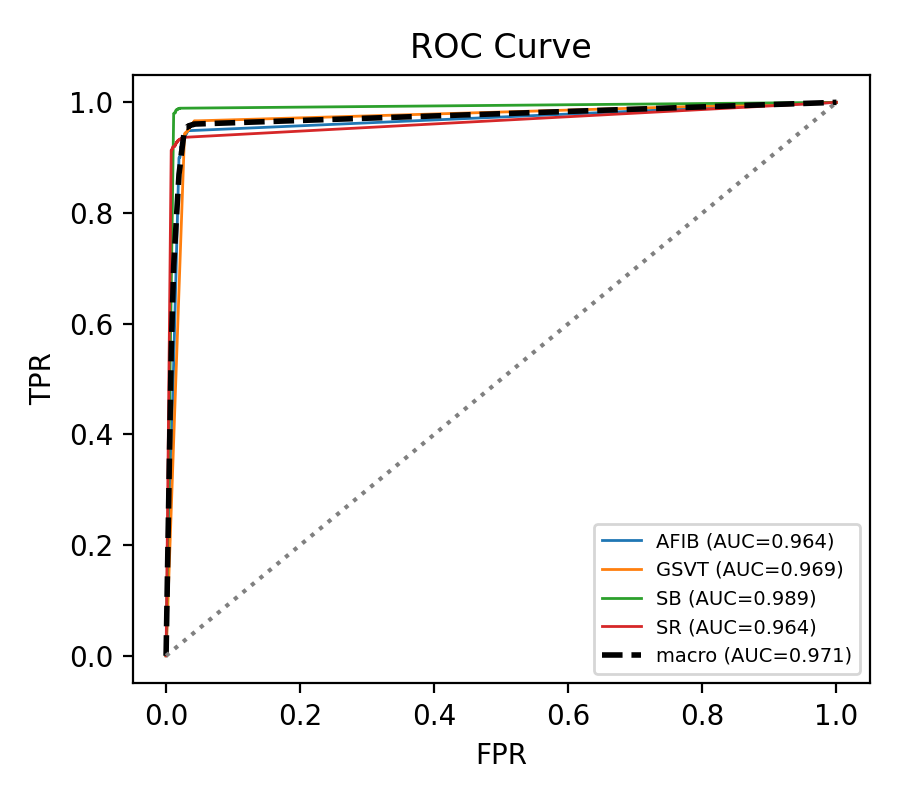
\includegraphics[width=\linewidth]{fig_roc_chapman.png}
  \caption{}
\end{subfigure}
\caption{Confusion matrix (a) and one-versus-rest ROC curves (b) of the INT8
model on the Chapman test set.}
\label{fig:chapman}
\end{figure}

Per-class results appear in Table~\ref{tab:perclass}. On Chapman, SB is the best
class, sinus bradycardia having a distinct rate signature; the hardest are GSVT
(precision 0.8698) and AFIB (recall 0.9062), the confusion matrix of
Fig.~\ref{fig:chapman}a showing AFIB taken for GSVT in 66 records and SR for GSVT
in 55. The macro-AUC of 0.971---0.989 for SB, 0.964 for AFIB and SR---indicates
that most remaining errors lie at the decision boundary between rhythm classes
rather than in poor separability.

Applied directly to Georgia with no retuning, the INT8 model attains 93.00\%
accuracy and 0.9151 macro-F1, about 1.3 points below the in-distribution result,
a modest degradation for a far-transfer setting across acquisition systems. The
float32 model scores 92.91\% and 0.9142 on the same set, so quantization is not
the source of the transfer loss; INT8--float32 prediction agreement is 0.9749.
\begin{figure}[t]
\centering
\begin{subfigure}{0.49\columnwidth}
  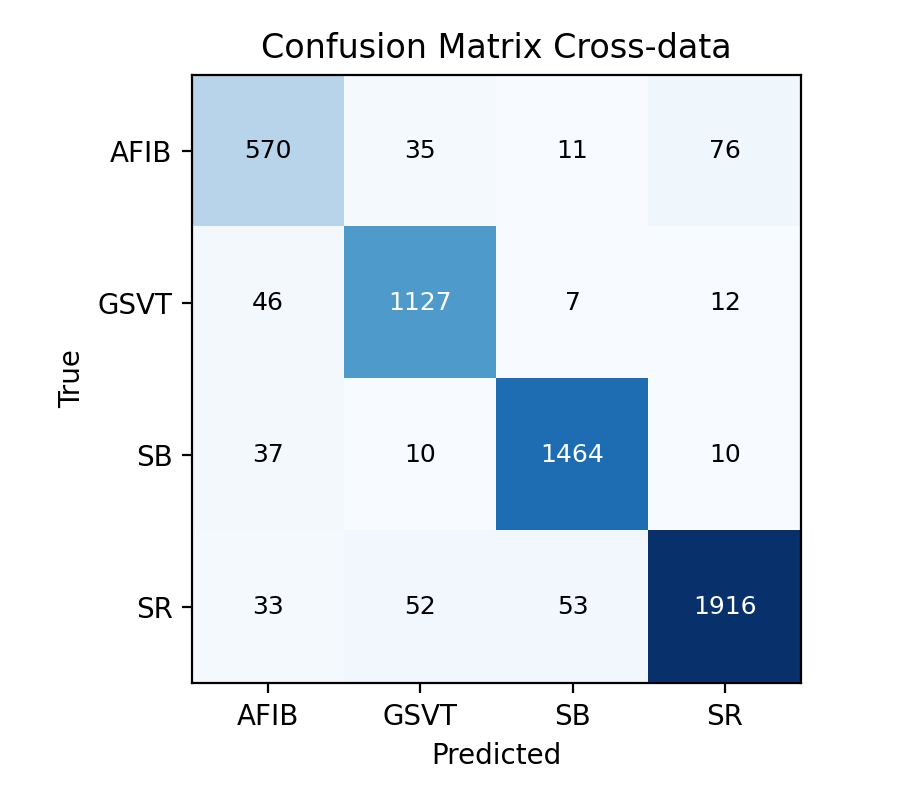
\includegraphics[width=\linewidth]{fig_cm_georgia.png}
  \caption{}
\end{subfigure}
\hfill
\begin{subfigure}{0.49\columnwidth}
  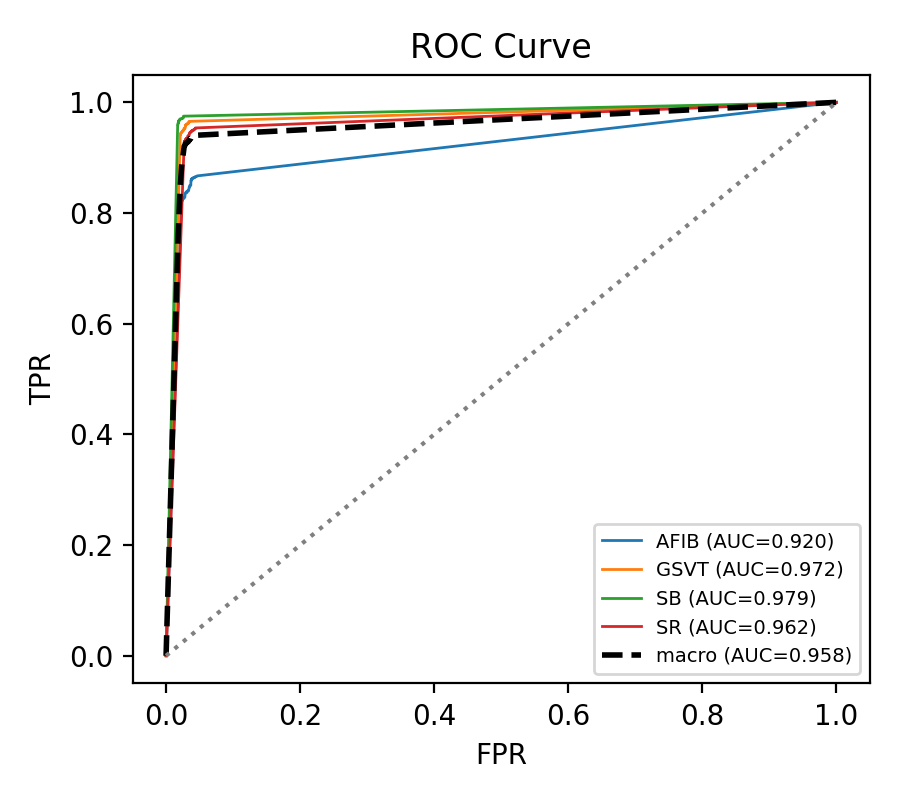
\includegraphics[width=\linewidth]{fig_roc_georgia.png}
  \caption{}
\end{subfigure}
\caption{Confusion matrix (a) and ROC curves (b) on the Georgia cross-dataset
test set, zero-shot with the Chapman weights.}
\label{fig:georgia}
\end{figure}

The macro-AUC is 0.958, with AFIB at 0.920 (Fig.~\ref{fig:georgia})---the lowest
of the four, yet far higher than its F1 of 0.8273 would suggest. A high AUC with a low F1 means the
model still ranks AFIB records correctly and that only the decision threshold
learned on Chapman is no longer optimal on the new distribution: the far-transfer
loss comes chiefly from a threshold shift, not from weaker feature recognition.

\subsection{Resources, Timing and Latency}

The design was synthesized with Quartus Prime 25.1 Lite for the Cyclone~V
5CSXFC6D6F31C6. Table~\ref{tab:res} gives the utilization. The engine unit
dominates, holding 24 of the 28 DSP blocks; the remaining four are in the FC
layer. The reported $F_{\max}$ at the slow corner (1100~mV, 85~$^\circ$C) is
108.86~MHz, with $+0.814$~ns of slack at the constrained frequency.

\begin{table}[t]
\caption{Resource utilization on the Cyclone~V 5CSXFC6D6F31C6.}
\label{tab:res}
\centering
\footnotesize
\begin{tabular}{lrrr}
\toprule
Resource & Used & Available & \% \\
\midrule
ALM               & 2{,}148 & 41{,}910 & 5 \\
Logic registers   & 2{,}902 & 83{,}820 & 3 \\
DSP blocks        & 28      & 112      & 25 \\
M10K blocks       & 20      & 553      & 4 \\
Block memory bits & 85{,}536 & 5{,}662{,}720 & 2 \\
\bottomrule
\end{tabular}
\end{table}

Because the controller has a fixed number of steps and no data-dependent branch,
the latency of one inference is constant. With the eight output channels running
in parallel, a convolutional layer takes $L_{\text{in}} \times C_{\text{in}}$
cycles for the main computation, giving 2{,}500, 2{,}000, 400 and 160 cycles for
Conv1--Conv4 and 22 for the output stage: 5{,}082 in total. Simulation measures
5{,}216. The 134-cycle difference is exactly the priming overhead: before a layer
yields its first result the window must be loaded with five values, each shift
costing $C_{\text{in}}$ cycles, to which 11 fixed cycles of pipeline depth and
pooling tail are added, so the overhead is $5C_{\text{in}}+11$, i.e. 16, 31, 31
and 51 cycles. Conv2--Conv4 match exactly; Conv1 measures one cycle more, bearing
also the transition from input loading, and 4 cycles remain for the state
transitions at either end and the bus latency of reading the status register.
At 100~MHz the 5{,}216 cycles give 52.16~$\mu$s and 19{,}172 inferences per
second (47.91~$\mu$s and 20{,}870~inferences/s at $F_{\max}$).

Power was estimated with the Quartus Power Analyzer from a switching-activity
file extracted from a full-system simulation: 536.08~mW total, of which
110.89~mW dynamic and 412.12~mW static, giving 27.96~$\mu$J per inference at
100~MHz. Section~\ref{sec:limits} qualifies this figure.

\subsection{On-Board Execution}

The bitstream was programmed onto a DE10-Standard kit, the host communicating
through the JTAG-to-Avalon bridge and System Console, with no operating system on
the board: a script writes the ECG samples into the input memory, asserts start,
waits for \texttt{done} and reads the class index. Over the complete Chapman test
set the board classifies 4{,}688 of 4{,}973 records correctly (94.27\%), and over
the complete Georgia set 5{,}077 of 5{,}459 (93.00\%). Both figures match the
software model exactly, as the bit-accurate verification predicts.

\subsection{Comparison with Related Work}

Table~\ref{tab:sota} compares the design with three FPGA accelerators for ECG
classification. Liu \emph{et al.} \cite{liu2023} is the closest comparison: same
dataset, same four rhythm groups, same record-level granularity and same
Cyclone~V family. Pham \emph{et al.} \cite{pham2025} and Tran \emph{et al.}
\cite{tran2026} classify individual beats on MIT-BIH, so their accuracy is not on
an equal footing: beat-level classification labels each beat, record-level labels
a whole ten-second segment, and the different unit means a different difficulty.

\begin{table}[t]
\caption{Comparison with related FPGA accelerators for ECG classification.}
\label{tab:sota}
\centering
\scriptsize
\setlength{\tabcolsep}{3pt}
\begin{tabular}{lcccc}
\toprule
 & \textbf{This work} & Liu \cite{liu2023} & Pham \cite{pham2025} & Tran \cite{tran2026} \\
\midrule
Device      & Cyclone V & Cyclone V & ZCU102 & Pynq-Z2 \\
Model       & 1D-CNN & 1D-CNN & Mini-Incep. & LDC \\
Parameters  & 640 & --- & 6{,}457 & --- \\
Quantization& INT8 & INT8 & fixed-16 & 1-bit \\
Dataset     & Chapman & Chapman & MIT-BIH & MIT-BIH \\
Granularity & rhythm & rhythm & beat & beat \\
Accuracy    & 94.27\% & 92.95\% & 99.37\% & 97.18\% \\
Logic       & 2{,}148 ALM (5\%) & 51\% & 24{,}685 LUT & 8{,}255 LUT \\
Registers   & 2{,}902 (3\%) & 86\% & 11{,}180 & 8{,}296 \\
DSP         & 28 (25\%) & 39\% & 40 & 0 \\
Frequency   & 100 MHz & 50 MHz & 250 MHz & 50 MHz \\
Latency     & 52.16 $\mu$s & 66 $\mu$s & 34.45 $\mu$s & 23.9 $\mu$s\textsuperscript{a} \\
Power       & 536.08 mW & 66 mW & 0.827 W & 1.709 W \\
\bottomrule
\end{tabular}
\\[2pt]
\raggedright\textsuperscript{a}\,Core only; 4{,}195 $\mu$s end-to-end.
\end{table}

Against the directly comparable design, the advantage is area together with
accuracy: 2{,}148 ALMs, 5\% of the device, and 3\% of the registers, against 51\%
and 86\%, at 94.27\% versus 92.95\% and a shorter latency despite the lower clock.
The difference is architectural. Liu \emph{et al.} map the whole network onto
hardware, trading area for latency, whereas replicating eight units along the
channel dimension and reusing them across layers keeps the area small while the
sequential schedule still fits the latency budget. The accuracy gap is consistent
with the rounding decision of Section~\ref{sec:quant}, though the two designs
differ in other respects as well and the comparison does not isolate that factor.
Power is not comparable in the same way: 66~mW in \cite{liu2023} is on a much
smaller device of the same family, and the static component dominates here
(Section~\ref{sec:limits}).

%=============================================================================
\section{Limitations}
\label{sec:limits}
%=============================================================================

The power and energy figures are estimates, not measurements. The 536.08~mW comes
from the Power Analyzer driven by a simulation activity file that does not cover
all combinational nodes, and the tool itself rates the confidence as low. The
number serves for relative comparison only. Moreover the static component is 77\%
of the total, a property of the large Cyclone~V device rather than of the design,
which makes the energy per inference look unfavourable against designs on smaller
parts; the core occupies 5\% of the logic, so most of that leakage is a cost of
the device.

The scope of the task is deliberately narrow: one lead, four rhythm groups and one
label per ten-second record, whereas clinical practice needs more disorders
distinguished, several of them recognizable only from multiple leads, and
record-level labelling cannot localize an abnormality within the segment. The
hardware configuration is fixed at synthesis---weights sit in on-chip ROM, so any
change of model requires resynthesis. Finally, data reach the board from a host
over the JTAG bridge, so the design is not yet coupled to an acquisition circuit
and has not been exercised on a continuous real-time stream with its far greater
noise and baseline wander.

%=============================================================================
\section{Conclusion}
%=============================================================================

This paper presented an FPGA accelerator for four-class ECG rhythm classification
built around two decisions. Power-of-two INT8 quantization with round-half-up
reduces rescaling to a constant addition and a bit shift, using no hard
multiplier, and the addition is absorbed into the accumulator initialization at no
cost on the critical path. Correctness is established by exact agreement with a
reference integer model at seven checkpoints spanning the network, not by
aggregate accuracy. The resulting core occupies 2{,}148 ALMs (5\%), 28 DSP blocks
and 20 M10K blocks on a Cyclone~V, closes timing at 108.86~MHz, and completes an
inference in a fixed 5{,}216 cycles---52.16~$\mu$s at 100~MHz. It reaches 94.27\%
accuracy and 0.9356 macro-F1 on Chapman and holds 93.00\% zero-shot on Georgia,
with the DE10-Standard bitstream reproducing both figures exactly.

Future work follows from the limitations: measuring supply-rail current during
continuous inference to bound the estimator's error and porting to a smaller
device of the same generation, where the leakage that now dominates is largely
absent; recalibrating decision thresholds on the target dataset, which the
AUC--F1 gap identifies as the main lever for far transfer; pipelining the layers
so that a later layer starts as soon as the previous has produced enough data;
and coupling the core to an acquisition front end with in-hardware filtering so
that it operates on a live stream.

%=============================================================================
\begin{thebibliography}{99}
\footnotesize

\bibitem{zheng2020}
J.~Zheng, J.~Zhang, S.~Danioko, H.~Yao, H.~Guo, and C.~Rakovski, ``A 12-lead
electrocardiogram database for arrhythmia research covering more than 10,000
patients,'' \emph{Scientific Data}, vol.~7, art.~48, 2020.

\bibitem{alday2020}
E.~A.~Perez Alday \emph{et al.}, ``Classification of 12-lead ECGs: the
PhysioNet/Computing in Cardiology Challenge 2020,'' \emph{Physiological
Measurement}, vol.~41, no.~12, art.~124003, 2020.

\bibitem{kiranyaz2016}
S.~Kiranyaz, T.~Ince, and M.~Gabbouj, ``Real-time patient-specific ECG
classification by 1-D convolutional neural networks,'' \emph{IEEE Trans. Biomed.
Eng.}, vol.~63, no.~3, pp.~664--675, 2016.

\bibitem{hannun2019}
A.~Y.~Hannun \emph{et al.}, ``Cardiologist-level arrhythmia detection and
classification in ambulatory electrocardiograms using a deep neural network,''
\emph{Nature Medicine}, vol.~25, no.~1, pp.~65--69, 2019.

\bibitem{le2023}
K.-H.~Le \emph{et al.}, ``LightX3ECG: A lightweight and explainable deep learning
system for 3-lead electrocardiogram classification,'' \emph{Biomed. Signal
Process. Control}, vol.~85, art.~104963, 2023.

\bibitem{yoon2023}
T.~Yoon and D.~Kang, ``Bimodal CNN for cardiovascular disease classification by
co-training ECG grayscale images and scalograms,'' \emph{Scientific Reports},
vol.~13, art.~2937, 2023.

\bibitem{li2017}
H.~Li, A.~Kadav, I.~Durdanovic, H.~Samet, and H.~P.~Graf, ``Pruning filters for
efficient ConvNets,'' in \emph{Proc. ICLR}, 2017.

\bibitem{jacob2018}
B.~Jacob \emph{et al.}, ``Quantization and training of neural networks for
efficient integer-arithmetic-only inference,'' in \emph{Proc. IEEE/CVF CVPR},
pp.~2704--2713, 2018.

\bibitem{miyashita2016}
D.~Miyashita, E.~H.~Lee, and B.~Murmann, ``Convolutional neural networks using
logarithmic data representation,'' arXiv:1603.01025, 2016.

\bibitem{bengio2013}
Y.~Bengio, N.~L\'eonard, and A.~Courville, ``Estimating or propagating gradients
through stochastic neurons for conditional computation,'' arXiv:1308.3432, 2013.

\bibitem{sze2017}
V.~Sze, Y.-H.~Chen, T.-J.~Yang, and J.~S.~Emer, ``Efficient processing of deep
neural networks: A tutorial and survey,'' \emph{Proc. IEEE}, vol.~105, no.~12,
pp.~2295--2329, 2017.

\bibitem{zhang2015}
C.~Zhang, P.~Li, G.~Sun, Y.~Guan, B.~Xiao, and J.~Cong, ``Optimizing FPGA-based
accelerator design for deep convolutional neural networks,'' in \emph{Proc.
ACM/SIGDA FPGA}, pp.~161--170, 2015.

\bibitem{venieris2018}
S.~I.~Venieris, A.~Kouris, and C.-S.~Bouganis, ``Toolflows for mapping
convolutional neural networks on FPGAs: A survey and future directions,''
\emph{ACM Computing Surveys}, vol.~51, no.~3, art.~56, 2018.

\bibitem{liu2023}
Y.~Liu \emph{et al.}, ``A fully-mapped and energy-efficient FPGA accelerator for
dual-function AI-based analysis of ECG,'' \emph{Frontiers in Physiology},
vol.~14, art.~1079503, 2023.

\bibitem{pham2025}
H.~L.~Pham, T.~D.~Tran, V.~T.~D.~Le, and Y.~Nakashima, ``MINA: A
hardware-efficient and flexible Mini-InceptionNet accelerator for ECG
classification in wearable devices,'' \emph{IEEE Trans. Circuits Syst. I},
vol.~72, no.~6, pp.~2740--2753, 2025.

\bibitem{tran2026}
A.~Tran, K.~Tran, and C.~Do, ``ECG-LDC: A hardware-efficient low-dimensional
computing framework for ECG arrhythmia classification,'' arXiv:2607.09680, 2026.

\end{thebibliography}

\end{document}
